%% LyX 2.2.3 created this file.  For more info, see http://www.lyx.org/.
%% Do not edit unless you really know what you are doing.
\documentclass[english,12pt]{article}
\usepackage[T1]{fontenc}
\usepackage[latin9]{inputenc}
\usepackage{float}
\usepackage{mathtools}
\usepackage{amsmath}
\usepackage{amsthm}
\usepackage{amssymb}
\usepackage{graphicx}

\makeatletter
%%%%%%%%%%%%%%%%%%%%%%%%%%%%%% Textclass specific LaTeX commands.
\theoremstyle{plain}
\newtheorem{thm}{\protect\theoremname}[section]
\theoremstyle{plain}
\newtheorem{prop}[thm]{\protect\propositionname}
\theoremstyle{definition}
\newtheorem{example}[thm]{\protect\examplename}
\theoremstyle{definition}
\newtheorem{defn}[thm]{\protect\definitionname}
\ifx\proof\undefined
\newenvironment{proof}[1][\protect\proofname]{\par
\normalfont\topsep6\p@\@plus6\p@\relax
\trivlist
\itemindent\parindent
\item[\hskip\labelsep\scshape #1]\ignorespaces
}{%
\endtrivlist\@endpefalse
}
\providecommand{\proofname}{Proof}
\fi
\theoremstyle{remark}
\newtheorem{rem}[thm]{\protect\remarkname}

%%%%%%%%%%%%%%%%%%%%%%%%%%%%%% User specified LaTeX commands.
\usepackage[margin=1in]{geometry}

\makeatother

\usepackage{babel}
\providecommand{\definitionname}{Definition}
\providecommand{\examplename}{Example}
\providecommand{\propositionname}{Proposition}
\providecommand{\remarkname}{Remark}
\providecommand{\theoremname}{Theorem}

\begin{document}

\title{Math 525: Lecture 14}

\date{February 22, 2018}
\maketitle

\section{Tightness}

Last lecture, we discussed convergence in distribution, culminating
in Helly's theorem:
\begin{prop}[Helly's theorem]
 Let $(F_{n})_{n}$ be a sequence of distribution functions. Then,
there exists a subsequence $(n_{k})_{k}$ and a right continuous nondecreasing
function $F$ such that
\[
F_{n_{k}}(x)\rightarrow F(x)\text{ for all continuity points }x\text{ of }F.
\]
\end{prop}
The issue with the above is that $F$ need not be a distribution function:
\begin{example}
~
\begin{enumerate}
\item Let $X_{n}=n$. Then, $F_{n}(x)=I_{[n,\infty)}(x)$ and $F_{n}(x)\rightarrow0$
for all $x$.
\item Let $X_{n}=-n$. Then, $F_{n}(x)=I_{[-n,\infty)}(x)$ and $F_{n}(x)\rightarrow1$
for all $x$.
\end{enumerate}
Neither $F=0$ nor $F=1$ are distribution functions.
\end{example}
A criteria that ensures the limiting function is indeed a distribution
function is tightness:
\begin{defn}
Let $\{F_{\alpha}\}_{\alpha}$ be a family of distribution functions.
We say $\{F_{\alpha}\}_{\alpha}$ is \emph{tight} if for every $\epsilon>0$,
there exists $r$ sufficiently large such that
\[
F_{\alpha}(r)-F_{\alpha}(-r)\geq1-\epsilon
\]
for all $\alpha$.
\end{defn}
\begin{prop}
Suppose that $(F_{n})_{n}$ is a tight sequence of distribution functions.
Then, there exists a subsequence $(n_{k})_{k}$ and a distribution
function $F$ such that $F_{n_{k}}\Rightarrow F$.
\end{prop}
In other words, the space of distribution functions is \emph{sequentially
compact}.
\begin{proof}
By Helly's theorem, we can find a subsequence $(n_{k})_{k}$ and a
right continuous nondecreasing function $F$ such that 
\[
F_{n_{k}}(x)\rightarrow F(x)\text{ for all continuity points }x\text{ of }F.
\]
By tightness, we can find $r$ such that
\[
F_{n}(-r)+\left(1-F_{n}(r)\right)\leq\epsilon.
\]
Since $F_{n}(-r)$ and $1-F_{n}(r)$ are both nonnegative, this implies
\[
F_{n}(-r)\leq\epsilon\qquad\text{and}\qquad1-F_{n}(r)\leq\epsilon.
\]
Now, choose $x_{\epsilon}>r$ so that both $x_{\epsilon}$ and $-x_{\epsilon}$
are continuity points of $F$. Then,
\[
F(-x_{\epsilon})=\lim_{k}F_{n_{k}}(-x_{\epsilon})\leq\epsilon
\]
and
\[
1-F(x_{\epsilon})=\lim_{k}\left\{ 1-F_{n_{k}}(x_{\epsilon})\right\} \leq\epsilon.
\]
Since $\epsilon$ was arbitrary, this implies
\[
\lim_{x\rightarrow-\infty}F(x)=0\qquad\text{and}\qquad\lim_{x\rightarrow\infty}F(x)=1,
\]
as desired.
\end{proof}

\section{Integration}

We will work a lot with integrals today, so let's digress and briefly
talk about integration. Suppose $f\colon\mathbb{R}\rightarrow\mathbb{R}$
is a continuous function. Then, the integral
\[
\int_{a}^{b}f(t)dt
\]
can be interpreted as the limit of Riemann sums. 
\begin{figure}[H]
\centering{}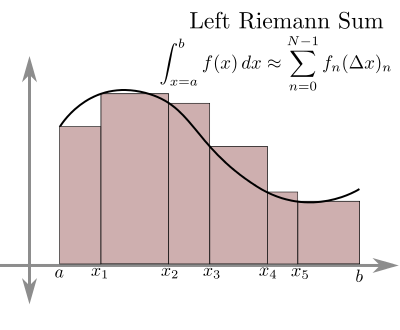
\includegraphics[height=3in]{riemann}
\end{figure}
What about when $f$ is not a ``nice'' function? Let $Y\sim U[0,1]$
and define
\[
\int_{a}^{b}f(t)dt\equiv\left(b-a\right)\mathbb{E}\left[f(Y)\right].
\]
The above extends the theory of integration to Borel measurable functions
$f$ (recall that if $f$ is Borel measurable, $f\circ Y$ is a random
variable). You can check that the definition of the integral above
satisfies all the usual conditions (e.g., linearity) and agrees with
the Riemann integral when $f$ is ``nice''.
\begin{rem}
You may have seen the Lebesgue integral. The above is not quite the
Lebesgue integral, since it is only defined for Borel measurable functions
$f$. 
\end{rem}
The above tells us that we can apply things like the Monotone Convergence
Theorem, Fatou's Lemma, and the Dominated Convergence Theorem to regular
integrals by treating them like expectations!

\section{L�vy's continuity theorem}

Our next goal is to establish Paul L�vy's continuity theorem, which
(roughly speaking) estabishes that a sequence of random variables
converges in distribution if and only if their characteristic functions
converge pointwise.

\subsection{Forward direction}

We have already done all the hard work to prove the forward direction.
\begin{prop}
\label{prop:forward}If $X_{n}\xrightarrow{\mathcal{D}}X$ (i.e.,
$F_{n}\Rightarrow F$) then $\mathbb{E}[e^{itX_{n}}]\equiv\phi_{n}(t)\rightarrow\phi(t)\equiv\mathbb{E}[e^{itX}]$
for all $t$.
\end{prop}
\begin{proof}
Remember that convergence in distribution was equivalent to
\[
\mathbb{E}\left[f(X_{n})\right]\rightarrow\mathbb{E}\left[f(X)\right]
\]
for all bounded and continuous $f$. Let $t$ be arbitrary and take
$f(x)=e^{itx}$ so that
\[
\phi_{n}(t)=\mathbb{E}\left[e^{itX_{n}}\right]\rightarrow\mathbb{E}\left[e^{itX}\right]=\phi(t).\qedhere
\]
\end{proof}

\subsection{Reverse direction}

The remainder of this section is dedicated to proving the reverse
direction. Before we do so, let $X$ be a random variable and $\phi$
its characteristic function. Then, for any $T>0$,
\begin{multline*}
\frac{1}{2T}\int_{-T}^{T}\phi(t)dt=\frac{1}{2T}\int_{-T}^{T}\mathbb{E}\left[e^{itX}\right]dt\\
=\frac{1}{2T}\mathbb{E}\left[\int_{-T}^{T}e^{itX}dt\right]=\frac{1}{2T}\mathbb{E}\left[\frac{2\sin(TX)}{X}\right]=\mathbb{E}\left[\frac{\sin(TX)}{TX}\right]
\end{multline*}
where we have used the Fubini-Tonelli theorem to move the integration
into the expectation (take this as fact if you have yet to encounter
Fubini-Tonelli). Now, let $A>0$ and note that if $|x|>2A$, then
\[
\left|\frac{\sin(Tx)}{Tx}\right|\leq\frac{1}{2TA}.
\]
Let $B=\{-2A<X\leq2A\}$. Then, 
\begin{align*}
\left|\mathbb{E}\left[\frac{\sin(TX)}{TX}\right]\right| & \leq\mathbb{E}\left[\left|\frac{\sin(TX)}{TX}\right|I_{B}+\left|\frac{\sin(TX)}{TX}\right|I_{B^{c}}\right]\\
 & \leq\mathbb{E}\left[I_{B}+\frac{1}{2TA}I_{B^{c}}\right]\\
 & =\left(F(2A)-F(-2A)\right)+\frac{1-\left(F(2A)-F(-2A)\right)}{2TA}\\
 & =\left(1-\frac{1}{2TA}\right)\left(F(2A)-F(-2A)\right)+\frac{1}{2TA}.
\end{align*}
Now, take $T=1/A$ to get
\[
\frac{A}{2}\left|\int_{-1/A}^{1/A}\phi(t)dt\right|\leq\frac{1}{2}\left(F(2A)-F(-2A)\right)+\frac{1}{2}.
\]
Some algebra reveals
\begin{equation}
A\left|\int_{-1/A}^{1/A}\phi(t)dt\right|-1\leq F(2A)-F(-2A).\label{eq:tightness_criterion}
\end{equation}
In particular, (\ref{eq:tightness_criterion}) gives a criterion for
tightness in terms of characteristic functions:
\begin{prop}
\label{prop:tightness_criterion}Let $(X_{n})_{n}$ be a sequence
of random variables with distribution and characteristic functions
$F_{n}$ and $\phi_{n}$. The sequence $(F_{n})_{n}$ is tight if
for all $\epsilon>0$, there exists $\delta>0$ such that
\[
\frac{1}{\delta}\left|\int_{-\delta}^{\delta}\phi_{n}(t)dt\right|-1\geq1-\epsilon.
\]
\end{prop}
\begin{proof}
Take $A=1/\delta$ in (\ref{eq:tightness_criterion}).
\end{proof}
We are now ready to prove the reverse direction.
\begin{prop}[L�vy's continuity theorem]
 Let $(F_{n})_{n}$ be a sequence of distribution functions and $\phi_{n}$
be the characteristic function of $F_{n}$. Suppose $\phi_{n}\rightarrow\phi$
pointwise for some function $\phi$ which is continuous at the origin
($t=0$). Then, there exists a distribution function $F$ such that
$F_{n}\Rightarrow F$ and $\phi$ is the characteristic function of
$F$.
\end{prop}
Some notes:
\begin{itemize}
\item When we say ``$\phi$ is the characteristic function of $F$'',
we mean that a random variable $X$ associated to $F$ (e.g., take
$X=F^{-1}(Y)$ where $Y\sim U[0,1]$) has characteristic function
$\phi$.
\item That $\phi$ is a characteristic function is one of the results of
the theorem (the limit of characteristic functions need not be a characteristic
function in general).
\end{itemize}
\begin{proof}
Since $\phi$ is continuous at zero, we can choose $\delta$ small
enough so that
\[
\left|\phi(t)-1\right|<\epsilon/4\qquad\text{whenever }\left|t\right|<\delta.
\]
Now, for $Y\sim U[-\delta,\delta]$,
\[
\frac{1}{\delta}\int_{-\delta}^{\delta}\phi_{n}(t)dt\equiv2\mathbb{E}\left[\phi_{n}(Y)\right]\rightarrow2\mathbb{E}\left[\phi(Y)\right]\equiv\frac{1}{\delta}\int_{-\delta}^{\delta}\phi(t)dt
\]
by the DCT. Therefore, we can choose $N$ large enough such that for
all $n\geq N$,
\[
\frac{1}{\delta}\left|\int_{-\delta}^{\delta}\phi_{n}(t)-\phi(t)dt\right|<\frac{\epsilon}{2}.
\]
Next, note that
\begin{align*}
\frac{1}{\delta}\left|\int_{-\delta}^{\delta}\phi(t)dt\right| & =\frac{1}{\delta}\left|\int_{-\delta}^{\delta}\phi(t)-\phi_{n}(t)+\phi_{n}(t)dt\right|\\
 & \leq\frac{1}{\delta}\left|\int_{-\delta}^{\delta}\phi(t)-\phi_{n}(t)dt\right|+\frac{1}{\delta}\left|\int_{-\delta}^{\delta}\phi_{n}(t)dt\right|\\
 & <\frac{\epsilon}{2}+\frac{1}{\delta}\left|\int_{-\delta}^{\delta}\phi_{n}(t)dt\right|.
\end{align*}
Recalling that $|\phi(t)-1|<\epsilon/2$ for all $t\in[-\delta,\delta]$,
it follows that
\[
\frac{1}{\delta}\left|\int_{-\delta}^{\delta}\phi(t)dt\right|\equiv2\left|\mathbb{E}\left[\phi(Y)\right]\right|>2\left(1-\frac{\epsilon}{4}\right)=2-\frac{\epsilon}{2}.
\]
Therefore,
\[
2-\frac{\epsilon}{2}<\frac{1}{\delta}\left|\int_{-\delta}^{\delta}\phi(t)dt\right|<\frac{\epsilon}{2}+\frac{1}{\delta}\left|\int_{-\delta}^{\delta}\phi_{n}(t)dt\right|.
\]
Simplying,
\[
2-\epsilon<\frac{1}{\delta}\left|\int_{-\delta}^{\delta}\phi_{n}(t)dt\right|.
\]

By Proposition \ref{prop:tightness_criterion}, the sequence $(F_{n})_{n}$
is tight. By Helly's theorem, there exists a subsequence $(F_{n_{k}})_{k}$
and a distribution function $F$ such that $F_{n_{k}}\Rightarrow F$.
Let $\tilde{\phi}$ be the characteristic function of $F$. Then,
by Proposition \ref{prop:forward}, $\phi_{n_{k}}\rightarrow\tilde{\phi}$
pointwise. But $\phi_{n}\rightarrow\phi$, and hence $\phi=\tilde{\phi}$.

It can be shown that $F_{n}\Rightarrow F$, but the proof requires
showing that convergence in distribution is metrizable, which is out
of the scope of this course.
\end{proof}
We can finally return to a claim we made a long time ago about the
relationship between Poisson and Binomial random variables:
\begin{example}
The characteristic function of $\operatorname{Poisson}(\lambda)$
is
\[
\phi_{\operatorname{Poisson}(\lambda)}(t)=\exp\left(\lambda\left(e^{it}-1\right)\right).
\]
The characteristic function of $B(n,p_{n})$ is
\[
\phi_{B(n,p_{n})}(t)=\left(\left(1-p_{n}\right)+p_{n}e^{it}\right)^{n}.
\]
Suppose $np_{n}\rightarrow\lambda$ as $n\rightarrow\infty$. Then,
\[
\left(\left(1-p_{n}\right)+p_{n}e^{it}\right)^{n}=\left(1-np_{n}\left(e^{it}-1\right)\frac{1}{n}\right)^{n}\rightarrow\exp\left(\lambda\left(e^{it}-1\right)\right).
\]
\end{example}

\end{document}
